\documentclass[11pt,a4paper]{article}

\usepackage[a4paper,margin=1in]{geometry}
\usepackage{amsmath,amssymb,amsfonts,bm}
\usepackage{graphicx}
\usepackage{subcaption}
\usepackage{booktabs}
\usepackage{multirow}
\usepackage{array}
\usepackage{float}
\usepackage{placeins}
\usepackage{hyperref}
\usepackage{xcolor}
\usepackage{enumitem}
\usepackage{caption}

\hypersetup{
    colorlinks=true,
    linkcolor=blue!60!black,
    citecolor=blue!60!black,
    urlcolor=blue!60!black
}

\graphicspath{{figures/}{figures/optuna/}}

\newcommand{\epsbar}{\bar{\epsilon}}
\newcommand{\sigbar}{\bar{\sigma}}
\newcommand{\dt}{\Delta t}
\newcommand{\R}{\mathbb{R}}

\title{\textbf{Recurrent Constitutive Modelling of a Three-Phase Viscoelastic Composite}}
\author{}
\date{March 31, 2026}

\begin{document}
\maketitle

\section{Introduction}

This report studies the unit-cell problem posed in the coursework brief: a one-dimensional three-phase viscoelastic composite driven by a prescribed macroscopic strain history. The practical aim is to learn a macroscopic constitutive surrogate from data, while the scientific aim is to understand how much hidden state is actually required to represent the material memory.

The most direct answer to part (a) is that the macroscopic constitutive model takes the applied macroscopic strain history as input and returns the macroscopic stress history as output. In operator form,
\begin{equation}
\sigbar(t)=\mathcal{G}\!\left(\epsbar_{[0,t]}\right),
\label{eq:macro_operator}
\end{equation}
where $\epsbar_{[0,t]}$ denotes the strain history from time $0$ to time $t$. In discrete form, consistent with the supplied dataset,
\begin{equation}
\left\{\epsbar_n\right\}_{n=0}^{1000}\mapsto \left\{\sigbar_n\right\}_{n=0}^{1000}.
\label{eq:discrete_operator}
\end{equation}
The dataset contains only macroscopic strain and stress histories, so the task is not to identify microscopic fields or microscopic parameters directly. In particular, the report does \emph{not} treat the microscopic Young's moduli and viscosities of the three phases as supervised outputs. Instead, it learns a homogenised history-dependent constitutive law.

One important modelling note concerns the constitutive equation stated in the brief. The printed form uses a viscous term proportional to $\partial u/\partial t$, but for a Kelvin--Voigt-type constitutive law the physically consistent interpretation is a strain-rate term proportional to $\partial \epsilon/\partial t$. The implementation and the analysis therefore interpret the viscous response as strain-rate based, consistent with standard one-dimensional linear viscoelasticity.

The report is organised as a comparative investigation rather than a single-model demonstration. First, a data-driven architecture search is carried out over standard recurrent cells: vanilla RNN, GRU, and LSTM. Second, the hidden-variable question from part (c) is revisited using more physically structured recurrent neural operators inspired by the coursework skeleton and by the state-space formulation proposed by Liu et al.~\cite{Liu_2023}. This second stage is necessary because the first hidden-size sweep did not reveal a single dramatic threshold, and understanding \emph{why} that happened turns out to be one of the main results of the project.

\section{Problem Setup And Data}

The microscopic unit-cell problem is governed by kinematics, equilibrium, and a linear elastic-viscous constitutive law. In one dimension,
\begin{equation}
\epsilon(x,t)=\frac{\partial u(x,t)}{\partial x},
\label{eq:kinematic_relation}
\end{equation}
\begin{equation}
\frac{\partial \sigma(x,t)}{\partial x}=0,
\label{eq:equilibrium_relation}
\end{equation}
and, phasewise,
\begin{equation}
\sigma_i(t)=E_i\,\epsilon_i(t)+\eta_i\,\dot{\epsilon}_i(t),
\label{eq:kelvin_voigt_phase}
\end{equation}
where $E_i$ and $\eta_i$ are piecewise-constant material parameters for the three phases. Equation~\eqref{eq:equilibrium_relation} implies that the stress is uniform across the unit cell, while the phase strains remain distinct. For a three-phase series composite,
\begin{equation}
\sigbar(t)=\sigma_1(t)=\sigma_2(t)=\sigma_3(t),
\label{eq:uniform_stress}
\end{equation}
\begin{equation}
\epsbar(t)=f_1\epsilon_1(t)+f_2\epsilon_2(t)+f_3\epsilon_3(t),
\label{eq:macro_strain_average}
\end{equation}
with phase fractions $f_1+f_2+f_3=1$. Since each $\epsilon_i(t)$ evolves in time, the macroscopic law is history dependent even though each phase is linearly viscoelastic.

The dataset contains $400$ paired strain and stress histories, each sampled at $1001$ time points. A deterministic split with seed $20260328$ was used throughout: $280$ training samples, $60$ validation samples, and $60$ test samples. The time step is
\begin{equation}
\dt=\frac{1}{1000}=10^{-3}.
\label{eq:dt_definition}
\end{equation}
Train-only min--max scaling to the interval $[-1,1]$ was used for both input and output histories to prevent information leakage from the validation and test sets.

\begin{table}[t]
\centering
\caption{Dataset and preprocessing summary used throughout the study.}
\label{tab:data_summary}
\begin{tabular}{ll}
\toprule
Quantity & Value \\
\midrule
Total sequences & $400$ \\
Time steps per sequence & $1001$ \\
Training / validation / test split & $280/60/60$ \\
Time step $\dt$ & $10^{-3}$ \\
Input normalisation & Train-only min--max to $[-1,1]$ \\
Output normalisation & Train-only min--max to $[-1,1]$ \\
Loss used for model selection & MSE on normalised stress histories \\
Test metrics reported & RMSE, $R^2$, relative $L^2$ on raw stress \\
\bottomrule
\end{tabular}
\end{table}

Representative histories from the dataset are shown in Figure~\ref{fig:sample_histories}. The loading space is broad enough to contain monotonic, reversing, and cyclic-like trajectories, which makes hidden-state modelling non-trivial. The stress responses show pronounced hysteresis and lag, so a model that only uses the current strain value is not expected to be sufficient.

\begin{figure}[t]
\centering

\includegraphics[width=0.92\textwidth]{01_sample_histories.png}
\caption{Representative macroscopic strain and stress histories from the dataset. The responses are visibly history dependent and include both monotonic and reversing behaviour, motivating a recurrent constitutive model rather than an instantaneous stress--strain map.}
\label{fig:sample_histories}
\end{figure}

\FloatBarrier
\section{Methods}

\subsection{Cell-Based Recurrent Constitutive Models}

The first model family keeps the constitutive interface fixed and varies only the recurrent memory mechanism. At each time step $n$, the model is given the current strain, previous strain, and discrete strain rate:
\begin{equation}
\bm{\xi}_n=
\begin{bmatrix}
\epsbar_n\\
\epsbar_{n-1}\\
\dfrac{\epsbar_n-\epsbar_{n-1}}{\dt}
\end{bmatrix}.
\label{eq:step_features}
\end{equation}
These features are first mapped through a feature network,
\begin{equation}
\tilde{\bm{\xi}}_n=\phi(\bm{\xi}_n),
\label{eq:feature_network}
\end{equation}
and are then passed to a recurrent cell. For the vanilla RNN and GRU models the hidden update is
\begin{equation}
\bm{h}_n=\mathcal{C}\!\left(\tilde{\bm{\xi}}_n,\bm{h}_{n-1}\right),
\label{eq:cell_update}
\end{equation}
while for the LSTM the recurrent state is $(\bm{h}_n,\bm{c}_n)$, where $\bm{c}_n$ is the cell state. The predicted stress is read out from the same constitutive features together with the updated hidden state,
\begin{equation}
\hat{\sigbar}_n=\psi\!\left(\epsbar_n,\epsbar_{n-1},\frac{\epsbar_n-\epsbar_{n-1}}{\dt},\bm{h}_n\right).
\label{eq:cell_readout}
\end{equation}
This formulation makes the three architectures directly comparable: the difference lies in how memory is stored and updated, not in the outer stress readout.

The hidden state plays the role of a learned internal variable, but in the cell-based models this interpretation is only approximate. A GRU or LSTM can distribute memory across gates and channels in a way that is excellent for prediction but not directly tied to a specific physical state variable. This point becomes important later when the minimum hidden dimension is investigated.

\subsection{Training Procedure}

All models were trained with AdamW, learning-rate reduction on plateau, gradient clipping, and early stopping. The loss used during training and validation was the mean-squared error on the normalised stress histories, while all final metrics in the report are computed after inverse transforming the stresses back to physical units. The test relative $L^2$ error is
\begin{equation}
\frac{\lVert \hat{\bm{\sigma}}-\bm{\sigma}\rVert_2}{\lVert \bm{\sigma}\rVert_2},
\label{eq:relative_l2}
\end{equation}
where the vectors contain the full flattened raw stress histories excluding the first time step. The first stress value was pinned to the known target during training and standard evaluation so that the recurrent model was judged on the constitutive evolution rather than on a trivial initialisation mismatch. During free-running unseen-load inference, the first stress was instead estimated from a fitted initial-rate model.

\subsection{Hyperparameter Optimisation}

The cell-based models were tuned using Optuna~\cite{optuna_2019}. Thirty trials were run for each family with a Tree-structured Parzen Estimator sampler. The search space was:
\begin{itemize}[leftmargin=1.5em]
    \item batch size in $\{8,16,32\}$,
    \item learning rate in $[10^{-4},5\times 10^{-3}]$ on a log scale,
    \item weight decay in $[10^{-6},10^{-2}]$ on a log scale,
    \item gradient clip in $\{0.5,1.0,2.0,5.0\}$,
    \item hidden size in $\{4,8,\dots,48\}$,
    \item readout width in $\{64,96,128,192\}$,
    \item readout depth in $\{2,3,4\}$,
    \item feature width in $\{16,32,64,96\}$,
    \item feature depth in $\{1,2,3\}$.
\end{itemize}
The training budget was fixed at $220$ epochs with a minimum of $90$ epochs before early stopping, patience $60$, and a $\times 0.5$ learning-rate drop after $15$ stagnant epochs.

Figure~\ref{fig:optuna_search_summary} summarises the Optuna comparison, while Figure~\ref{fig:gru_optuna_detail} shows two important details for the winning GRU family: the training curves of the best trial and the parameter-importance estimate. The hidden dimension dominates the importance ranking, accounting for approximately $50.5\%$ of the estimated importance. That result already suggests that part (c) cannot be treated as an afterthought.

\begin{figure}[t]
\centering
\begin{subfigure}[t]{0.47\textwidth}
    \centering
    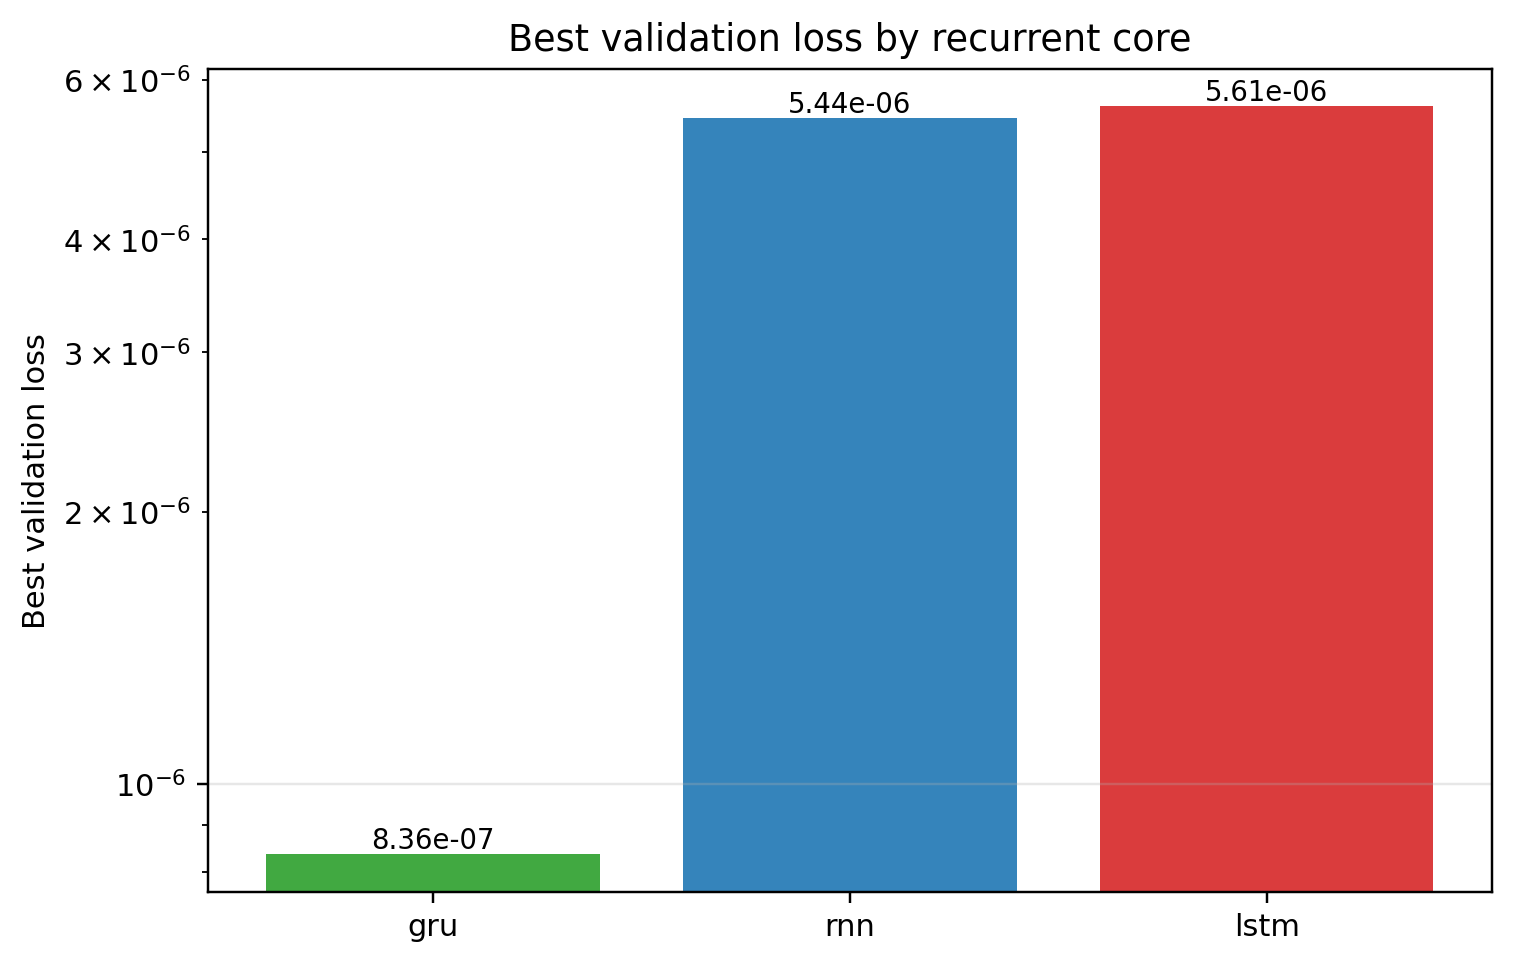
\includegraphics[width=\textwidth]{optuna/02_family_best_validation_loss.png}
    \caption{Best validation loss by cell family.}
\end{subfigure}
\hfill
\begin{subfigure}[t]{0.47\textwidth}
    \centering
    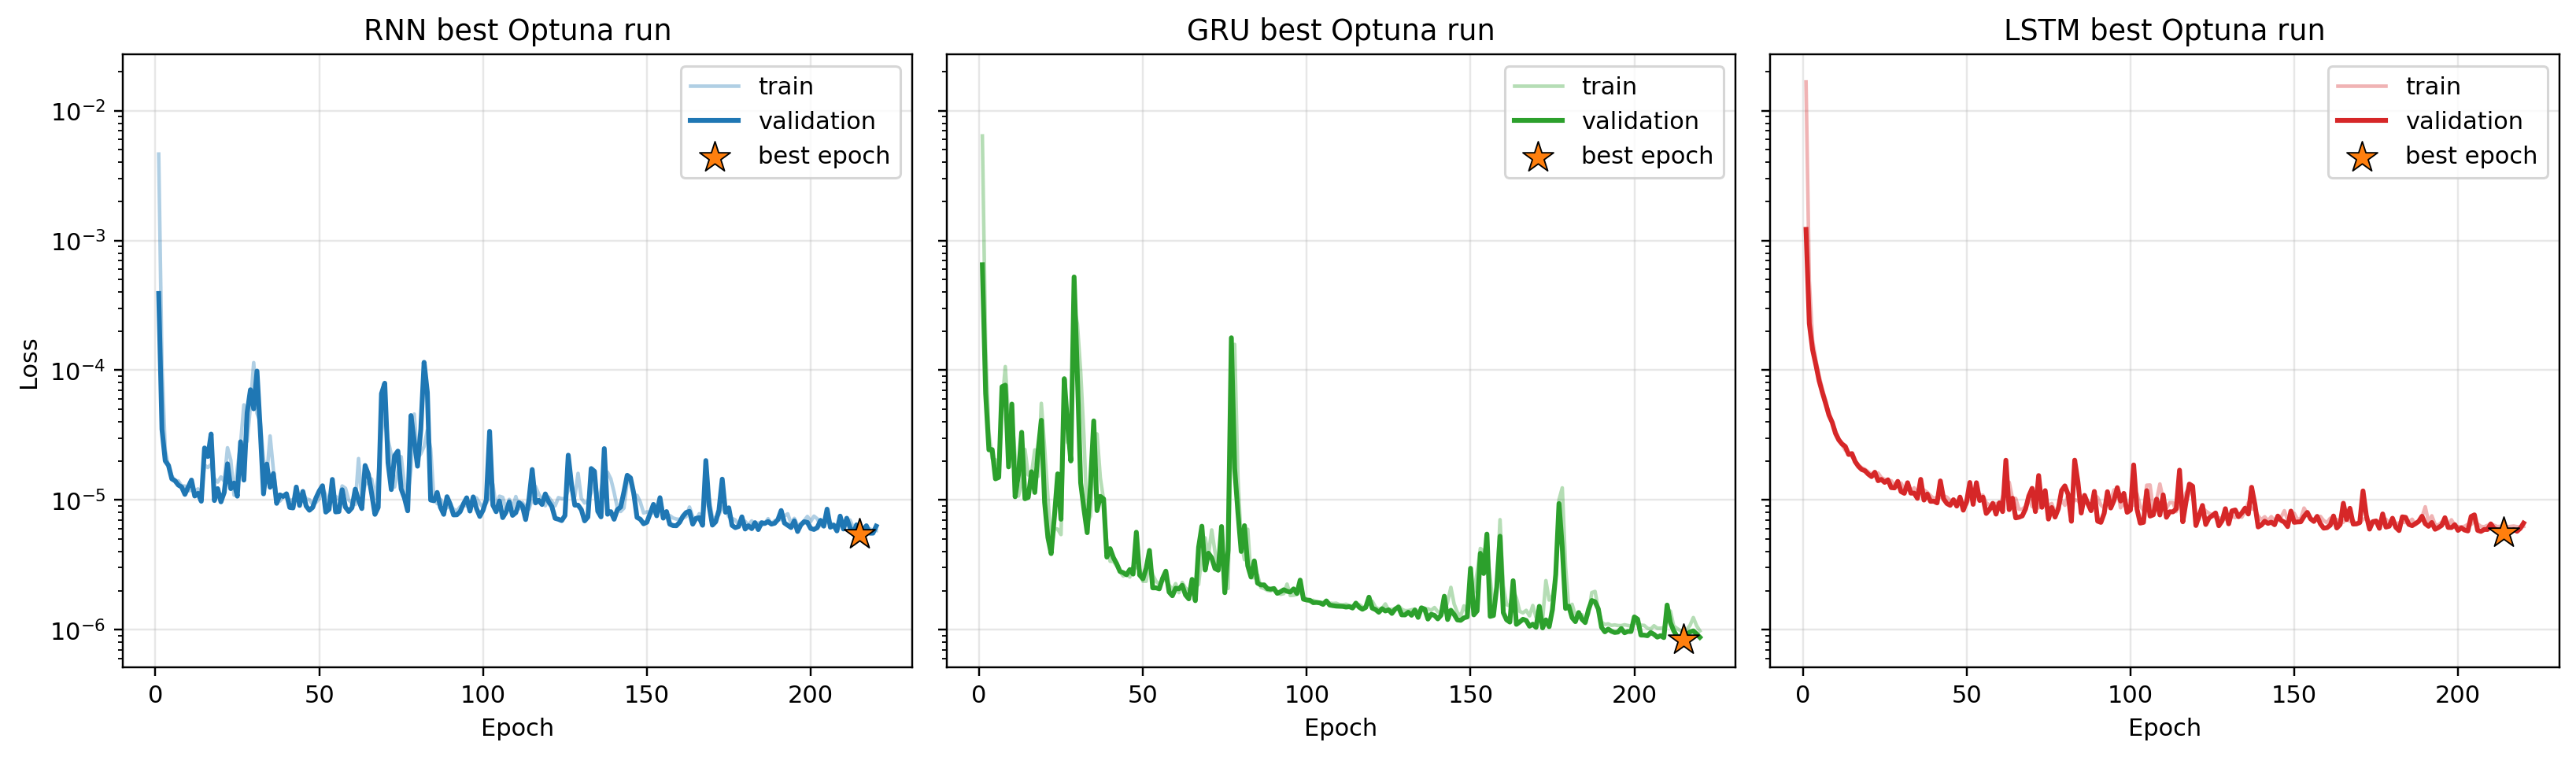
\includegraphics[width=\textwidth]{optuna/02_best_optuna_training_curves.png}
    \caption{Training and validation curves for the best trial in each family.}
\end{subfigure}
\caption{Optuna architecture search over vanilla RNN, GRU, and LSTM. GRU achieved the lowest validation loss by a clear margin, while LSTM plateaued earlier and at a higher loss despite having the most flexible gating mechanism.}
\label{fig:optuna_search_summary}
\end{figure}

\begin{figure}[t]
\centering
\begin{subfigure}[t]{0.47\textwidth}
    \centering
    
\includegraphics[width=\textwidth]{optuna/02_gru_param_importance.png}
    \caption{Optuna parameter importance for the GRU study.}
\end{subfigure}
\hfill
\begin{subfigure}[t]{0.47\textwidth}
    \centering
    
\includegraphics[width=\textwidth]{optuna/02_gru_loss_vs_hidden.png}
    \caption{GRU validation loss against hidden dimension across the Optuna trials.}
\end{subfigure}
\caption{Optimisation details for the winning GRU family. The hidden dimension is the dominant optimisation variable, while the trial scatter also shows that hidden-size effects are not perfectly sharp even before the more focused threshold studies.}
\label{fig:gru_optuna_detail}
\end{figure}

\FloatBarrier
\subsection{Operator-Inspired Recurrent Models}

The second model family was introduced to study hidden variables in a more explicitly state-space form, following the internal-variable viewpoint of Liu et al.~\cite{Liu_2023}. Two variants were used.

\paragraph{Baseline RNO.}
The first variant stays close to the coursework skeleton. Its hidden state evolves by an explicit Euler step,
\begin{equation}
\bm{h}_n=\bm{h}_{n-1}+\dt\,\bm{g}\!\left(\epsbar_{n-1},\bm{h}_{n-1}\right),
\label{eq:baseline_state_update}
\end{equation}
and the stress is read out from previous strain, discrete strain rate, and the hidden state,
\begin{equation}
\hat{\sigbar}_n=f\!\left(\epsbar_{n-1},\frac{\epsbar_{n-1}-\epsbar_n}{\dt},\bm{h}_{n-1}\right).
\label{eq:baseline_readout}
\end{equation}
This model is useful because it is much closer to the supplied RNO skeleton than the standard cell-based architectures.

\paragraph{Paper-inspired RNO.}
The second variant follows the cleaner state-space form proposed by Liu et al.~\cite{Liu_2023}. In its most general form,
\begin{equation}
\hat{\sigbar}_n=f\!\left(\epsbar_n,\dot{\epsbar}_n,\bm{h}_{n}\right),
\label{eq:paper_stress_relation}
\end{equation}
\begin{equation}
\bm{h}_{n}=\bm{h}_{n-1}+\dt\,\bm{g}\!\left(\epsbar_n,\bm{h}_{n-1}\right).
\label{eq:paper_kinetic_relation}
\end{equation}
Two cases were tested:
\begin{enumerate}[leftmargin=1.5em]
    \item \textbf{No-rate paper RNO:} the stress readout uses only $\epsbar_n$ and $\bm{h}_n$,
    \item \textbf{With-rate paper RNO:} the stress readout uses $\epsbar_n$, $\dot{\epsbar}_n$, and $\bm{h}_n$.
\end{enumerate}
The distinction is critical. In the no-rate model, the hidden state is forced to carry essentially all of the constitutive memory. In the with-rate model, part of the relevant physics is supplied explicitly through the strain-rate channel.

This separation is also relevant to the hidden-size question. If $h=0$ in the no-rate paper RNO, the constitutive law collapses to an instantaneous map
\begin{equation}
\hat{\sigbar}_n=f\!\left(\epsbar_n\right),
\label{eq:h0_no_rate}
\end{equation}
which is structurally incapable of representing a general history-dependent constitutive law. If $h=0$ in the with-rate model, the constitutive law becomes
\begin{equation}
\hat{\sigbar}_n=f\!\left(\epsbar_n,\dot{\epsbar}_n\right),
\label{eq:h0_with_rate}
\end{equation}
which is still memoryless in the latent sense, but is much stronger because the rate effect is supplied directly.

\FloatBarrier
\section{Results}

\subsection{Best Predictive Model From The Architecture Search}

Table~\ref{tab:model_comparison} summarises the best predictive model from each family together with the skeleton-faithful baseline RNO matched to the best GRU training recipe. The GRU achieved the lowest validation loss and the lowest test errors overall. Its test relative $L^2$ error was $3.72\times 10^{-3}$ and its coefficient of determination was $0.999986$, making it the strongest predictive model in the study.

\begin{table}[t]
\centering
\caption{Best predictive models. The test relative $L^2$ values are taken from the saved hidden-state analysis outputs so that every model is evaluated under the same raw-stress metric.}
\label{tab:model_comparison}
\begin{tabular}{lcccc}
\toprule
Model & Best val. loss & Test RMSE & Test relative $L^2$ & Test $R^2$ \\
\midrule
GRU & $8.36\times 10^{-7}$ & $1.26\times 10^{-3}$ & $3.72\times 10^{-3}$ & $0.999986$ \\
Baseline RNO & $4.73\times 10^{-6}$ & $2.87\times 10^{-3}$ & $8.46\times 10^{-3}$ & $0.999928$ \\
RNN & $5.44\times 10^{-6}$ & $3.02\times 10^{-3}$ & $8.91\times 10^{-3}$ & $0.999920$ \\
LSTM & $5.61\times 10^{-6}$ & $3.09\times 10^{-3}$ & $9.12\times 10^{-3}$ & $0.999916$ \\
\bottomrule
\end{tabular}
\end{table}

The dominance of the GRU is consistent with the training curves in Figure~\ref{fig:optuna_search_summary}. The LSTM did not outperform the GRU, even though it has the most expressive gating mechanism. The most plausible explanation is that the dataset is not large enough to reward the extra flexibility of a full cell-state architecture. The GRU appears to provide the best trade-off between memory capacity and optimisation difficulty. In contrast, the vanilla RNN is most exposed to gradient degradation over long sequences, and the LSTM pays a higher parameter and optimisation cost without a corresponding generalisation gain.

The baseline RNO sits between the GRU and the other cell-based models. This is an important result: a custom state-space constitutive operator can be competitive, but in this dataset the best purely predictive model is still the gated GRU. All final reported results were run on CPU; although Apple MPS was available, the explicit time-marching loop made CPU execution faster in practice for this workload.

\subsection{Qualitative Behaviour Of The Best GRU Model}

The best GRU was then evaluated on the held-out test set and on unseen cyclic loading. Figure~\ref{fig:qualitative_test_examples} shows best, median, and worst test trajectories in both stress--time and stress--strain space. Even the worst selected example remains physically plausible and follows the correct loop orientation, although the largest deviations occur around turning points and steep changes in slope. This is consistent with a recurrent model that has learned the broad constitutive structure but still accumulates its largest errors where history and rate interact most strongly.

\begin{figure}[t]
\centering
\begin{subfigure}[t]{0.48\textwidth}
    \centering
    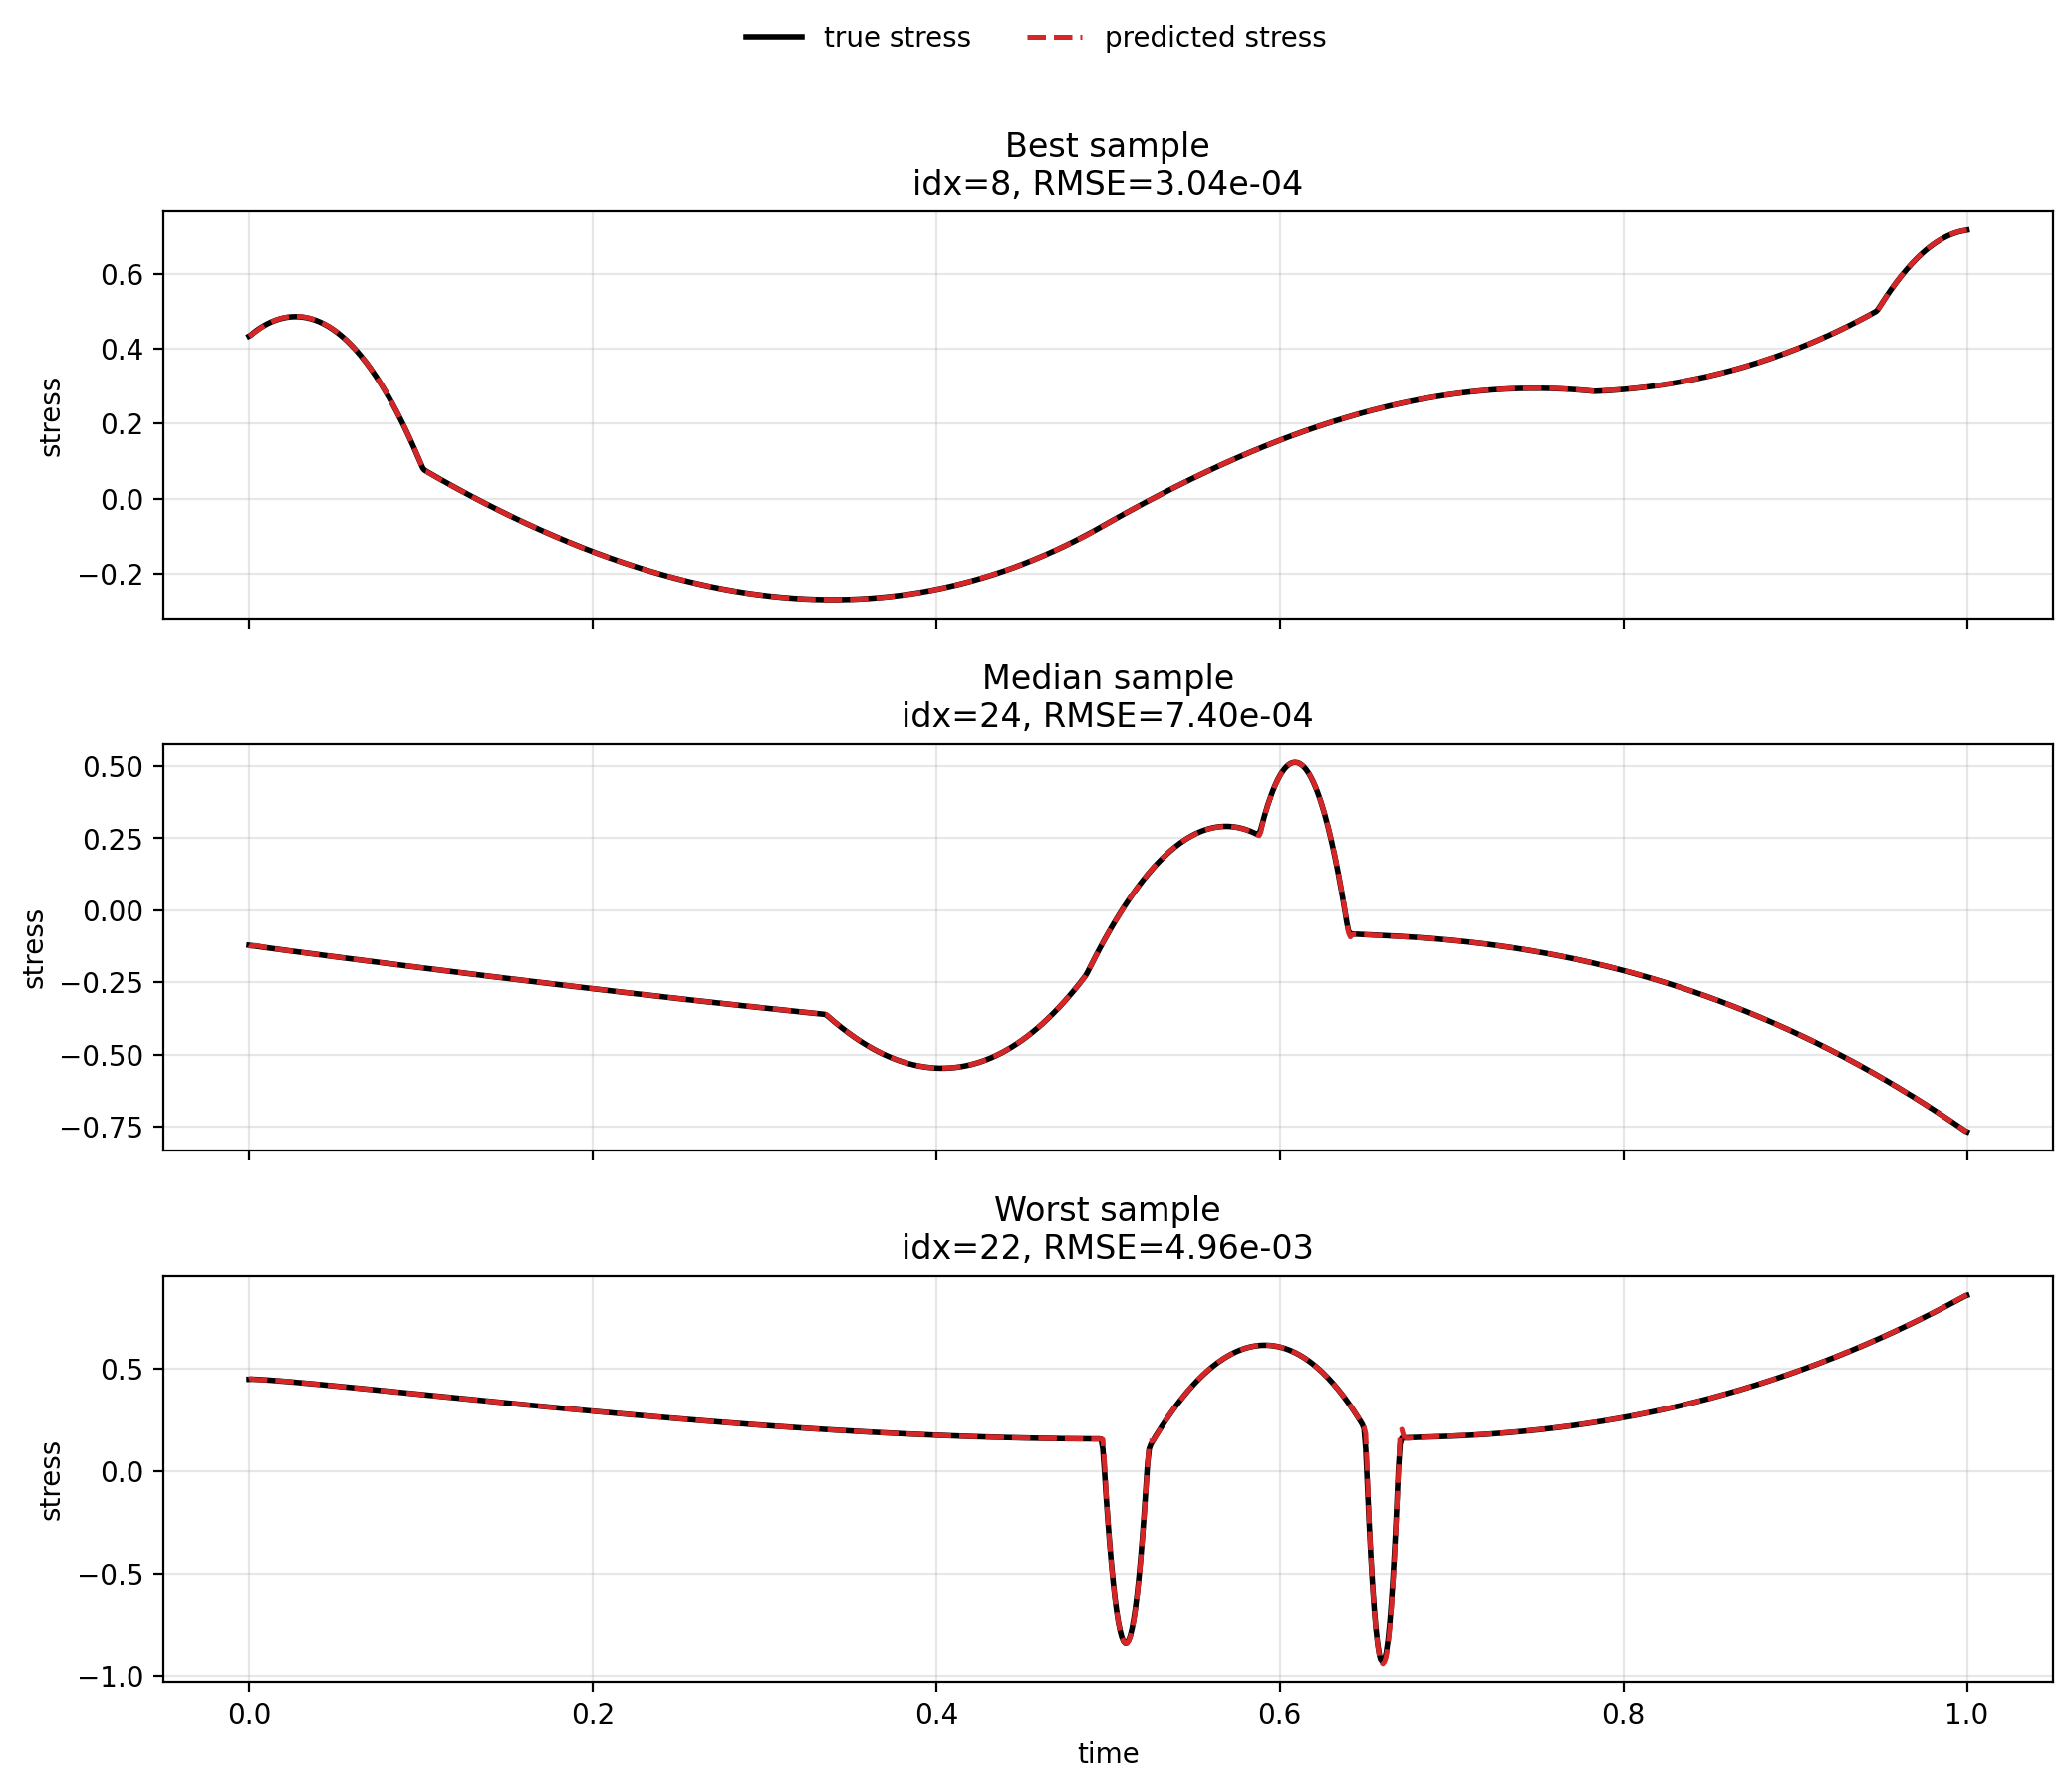
\includegraphics[width=\textwidth]{05_test_stress_time_examples.png}
    \caption{Stress histories in time for best, median, and worst test samples.}
\end{subfigure}
\hfill
\begin{subfigure}[t]{0.48\textwidth}
    \centering
    
\includegraphics[width=\textwidth]{05_test_stress_strain_examples.png}
    \caption{Stress--strain trajectories for the same three test samples.}
\end{subfigure}
\caption{Qualitative behaviour of the best Optuna GRU on the test set. The model captures the overall constitutive loops very well, while the remaining errors concentrate near sharp turning points and the highest-curvature portions of the trajectories.}
\label{fig:qualitative_test_examples}
\end{figure}

Figure~\ref{fig:hysteresis_and_residuals} complements these trajectory plots. The residual plot shows that the best GRU has small, mostly structureless errors on the test set, while the unseen cyclic tests show that the model reproduces hysteresis loops rather than collapsing to an elastic single-valued response. This matters because a visually good time-series fit alone would not prove that the model has learned a meaningful constitutive relation.

\begin{figure}[t]
\centering
\begin{subfigure}[t]{0.48\textwidth}
    \centering
    
\includegraphics[width=\textwidth]{04_residual_analysis.png}
    \caption{Residual analysis for the best GRU on the held-out test set.}
\end{subfigure}
\hfill
\begin{subfigure}[t]{0.48\textwidth}
    \centering
    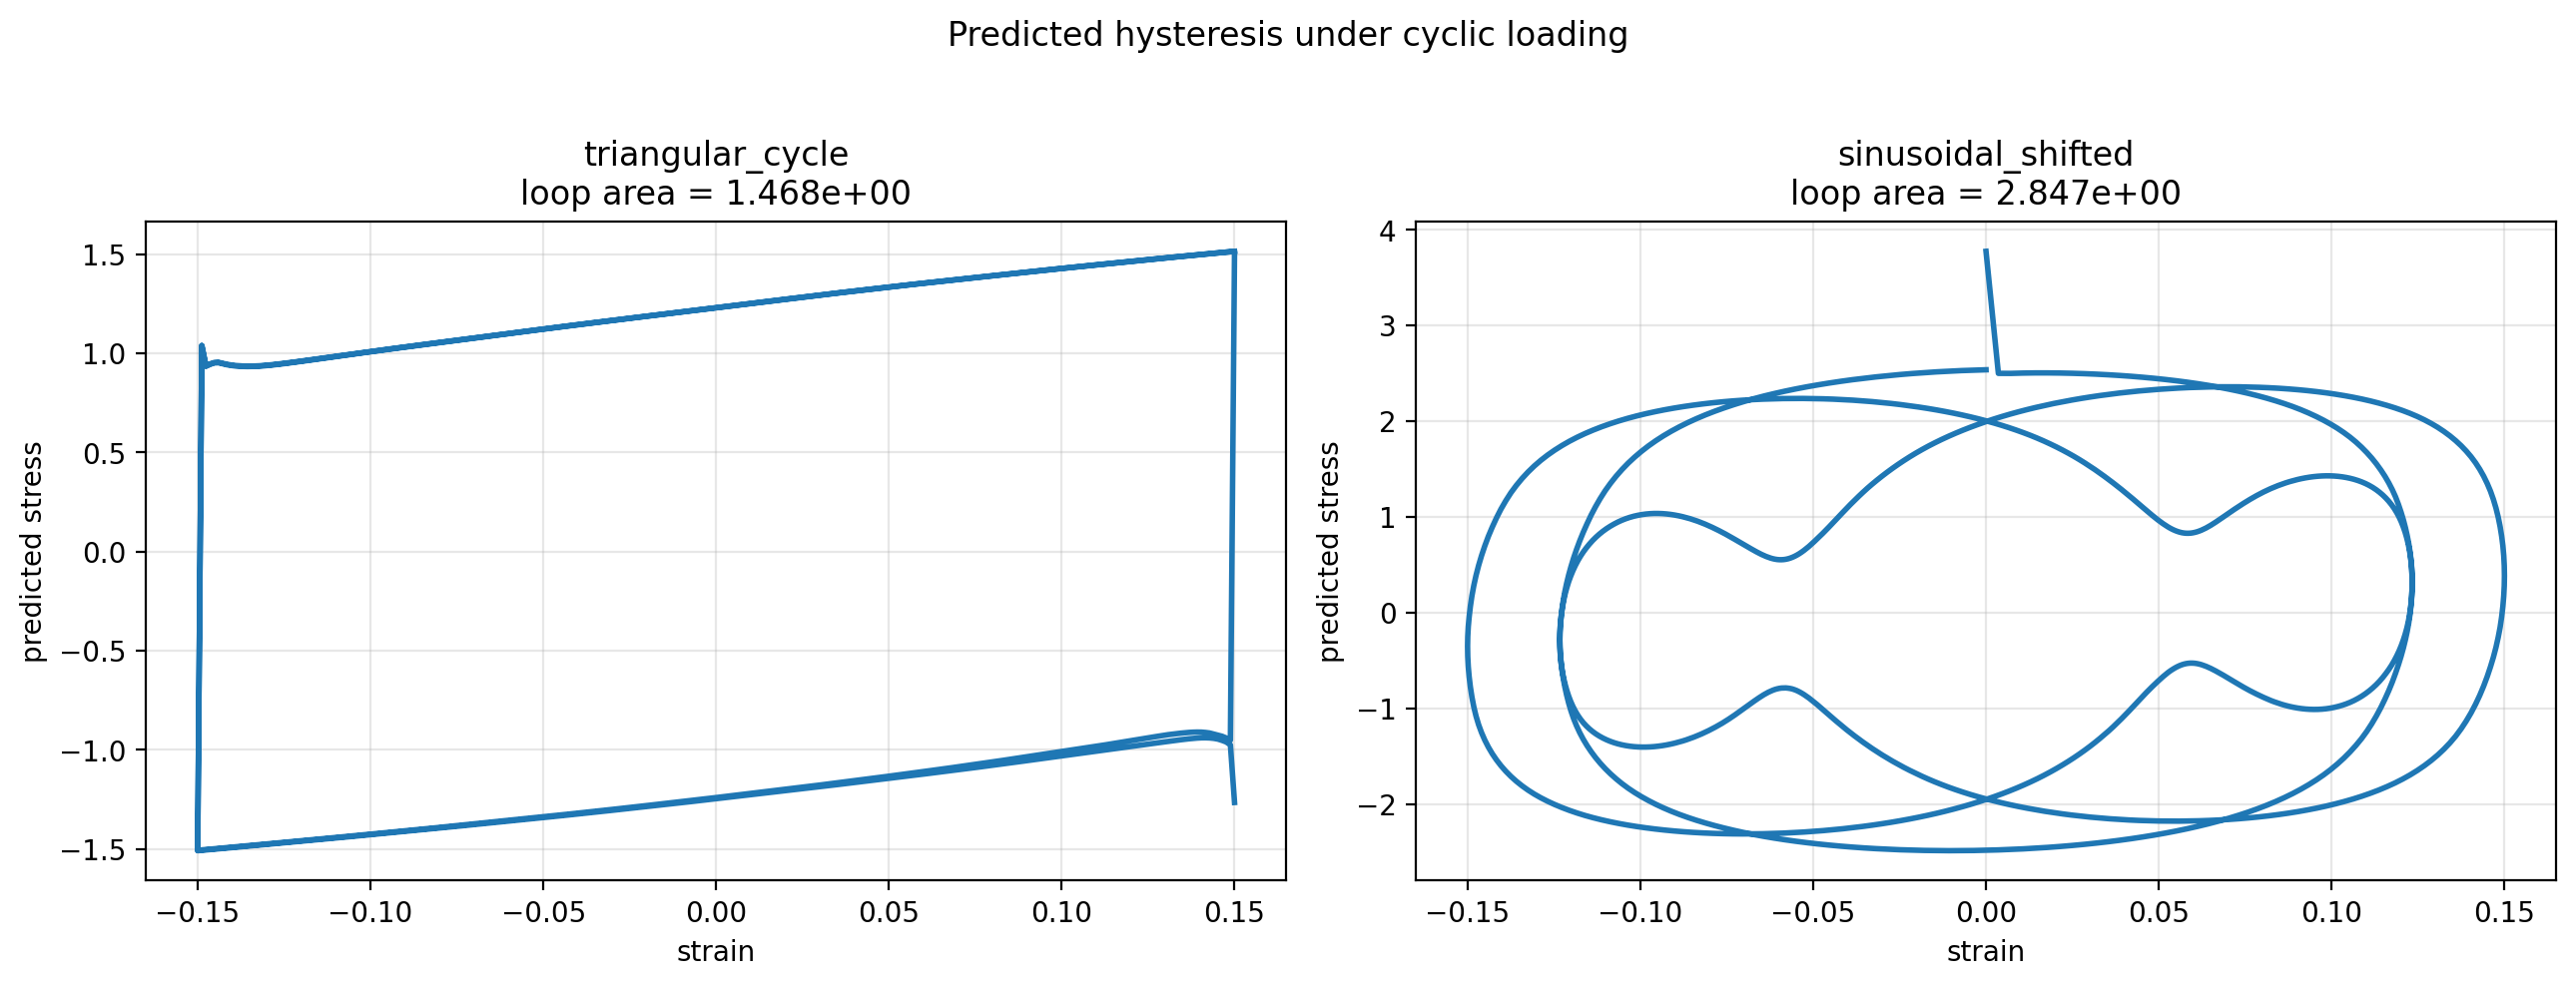
\includegraphics[width=\textwidth]{05_hysteresis_checks.png}
    \caption{Predicted hysteresis under unseen cyclic loading.}
\end{subfigure}
\caption{Additional qualitative checks for the best GRU. The residuals are small and unbiased overall, while the unseen cyclic tests demonstrate that the model reproduces looped, rate-dependent behaviour rather than a purely elastic stress--strain curve.}
\label{fig:hysteresis_and_residuals}
\end{figure}

\FloatBarrier
\subsection{Initial Hidden-Size Sweep On The Best GRU}

The first attempt to answer part (c) was to freeze the best non-hidden hyperparameters from the winning GRU and sweep the hidden size downward. The result is shown in Figure~\ref{fig:gru_threshold_attempt}. The key observation is that the error improves smoothly from $h=0$ to $h=4$ rather than exhibiting a dramatic cliff. The mean validation loss decreases from $8.38\times 10^{-6}$ at $h=0$ to $3.27\times 10^{-6}$ at $h=4$, but no value in the tested range reached the strict $5\%$ threshold relative to the Optuna-best GRU.

\begin{figure}[t]
\centering

\includegraphics[width=0.78\textwidth]{hidden_threshold_low_dim_with_reference_threshold.png}
\caption{Low-dimensional hidden-size sweep for the best GRU recipe, compared with the cached $h=4$ reference. The trend is monotonic but smooth, and no hidden size in $\{0,1,2,3,4\}$ met the strict $5\%$ threshold defined relative to the Optuna-best GRU result.}
\label{fig:gru_threshold_attempt}
\end{figure}

This apparently inconclusive result is already informative. In the GRU formulation, the model is given the explicit feature vector from Equation~\eqref{eq:step_features}, so the $h=0$ case is \emph{not} a truly memoryless constitutive law. Even without latent state, it still receives the current strain, previous strain, and discrete strain rate directly. That makes the zero-hidden case much stronger than the clean internal-variable test considered by Liu et al.~\cite{Liu_2023}, and it explains why the threshold is blurred rather than sharply exposed.

\subsection{Operator-Style Follow-Up For Part (c)}

Because the GRU threshold was not sharp, the hidden-variable study was extended to models with more explicit state evolution. The first decisive result is shown in Figure~\ref{fig:paper_h0_ablation}, where the paper-inspired RNO is tested at $h=0$ with and without explicit strain rate in the stress readout.

\begin{figure}[t]
\centering

\includegraphics[width=0.78\textwidth]{08_paper_rno_h0_comparison.png}
\caption{Paper-inspired $h=0$ ablation. Without explicit strain rate, the paper-style model fails badly. Adding the strain-rate channel recovers orders of magnitude of accuracy even though the latent hidden dimension remains zero.}
\label{fig:paper_h0_ablation}
\end{figure}

The numerical contrast is stark. For the no-rate paper RNO at $h=0$, the best validation loss is $3.98\times 10^{-2}$ and the test relative $L^2$ error is $0.721$. For the with-rate paper RNO at $h=0$, the best validation loss drops to $8.74\times 10^{-6}$ and the test relative $L^2$ error drops to $1.14\times 10^{-2}$. This is one of the most important findings in the report. A clean state-space model with no explicit rate input and no hidden state is structurally incapable of representing the constitutive law; once the rate channel is restored, much of the missing information is supplied explicitly and the apparent need for latent state becomes much weaker.

The full hidden-size sweeps for the paper-inspired models are shown in Figure~\ref{fig:paper_hidden_sweeps}. The no-rate model improves strongly from $h=0$ to $h=3$, after which it plateaus. The with-rate model starts from a much better $h=0$ baseline and improves more smoothly, reaching its best value at the edge of the tested range.

\begin{figure}[t]
\centering
\begin{subfigure}[t]{0.48\textwidth}
    \centering
    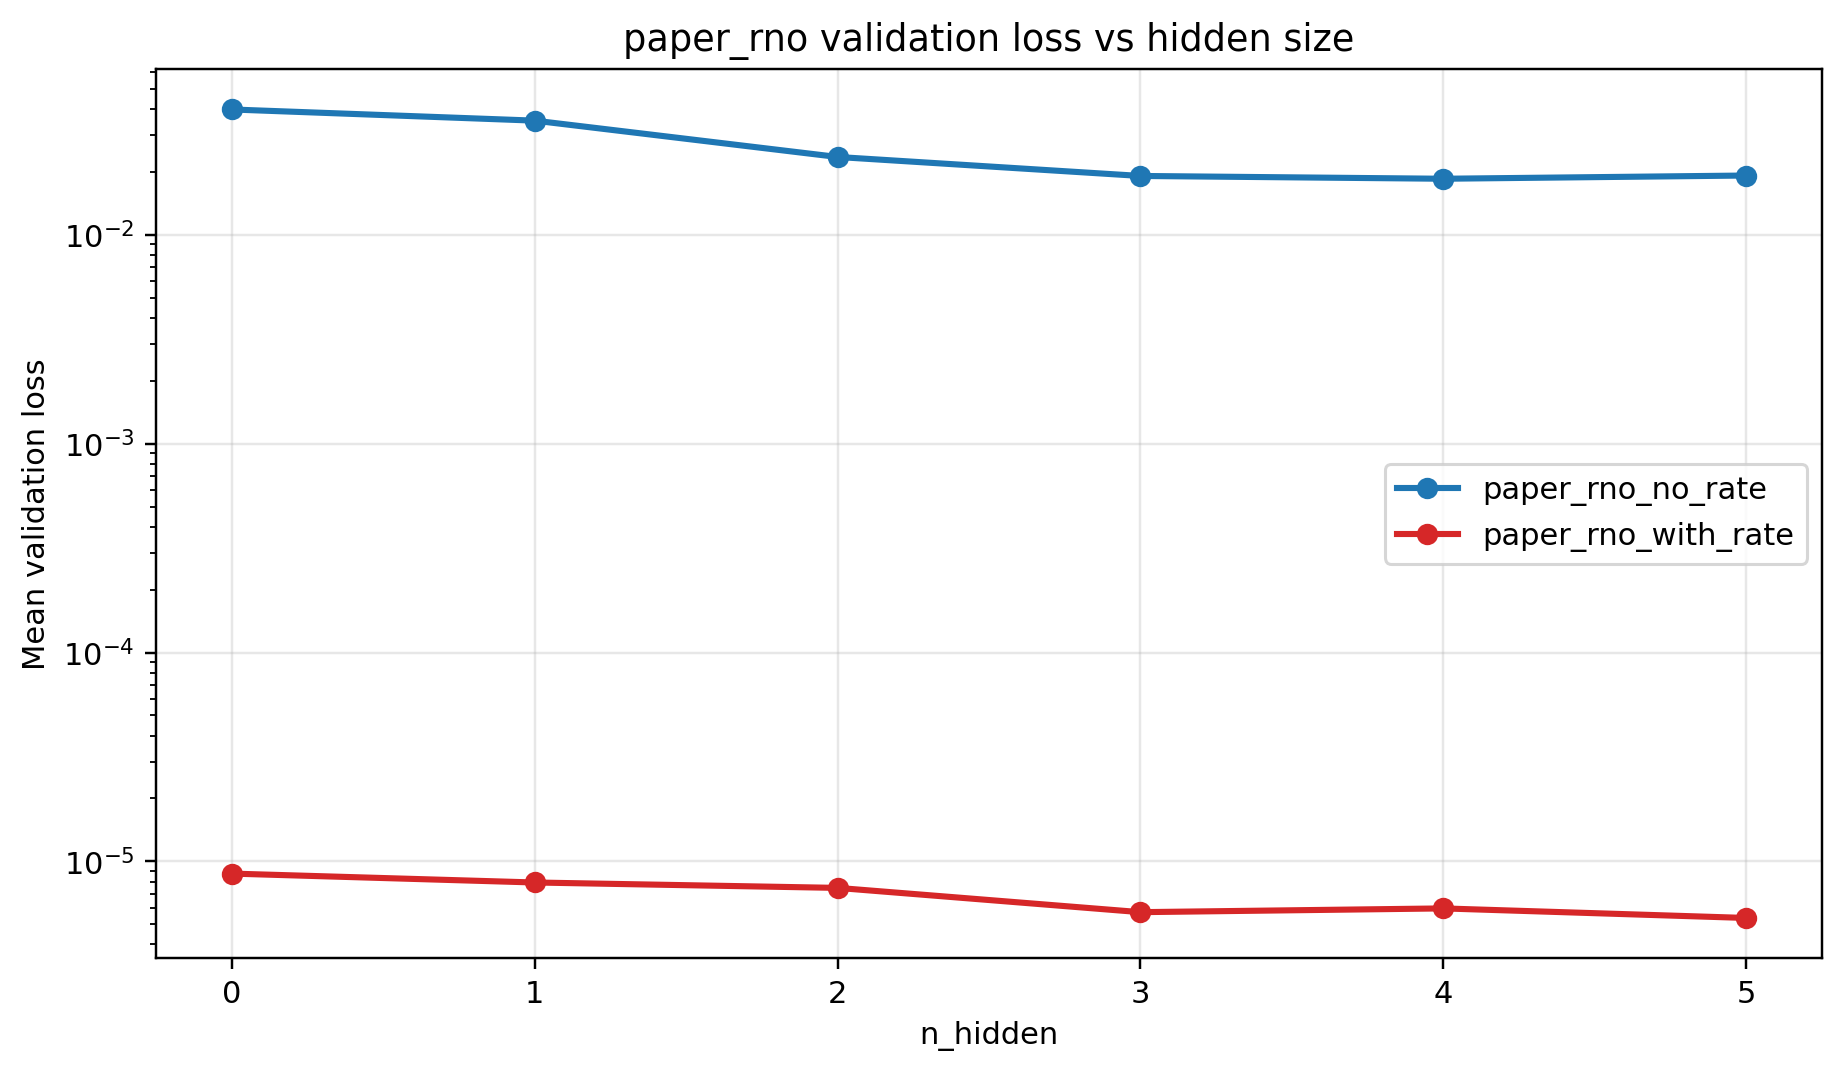
\includegraphics[width=\textwidth]{09_paper_rno_validation_loss_vs_hidden.png}
    \caption{Validation loss against hidden dimension.}
\end{subfigure}
\hfill
\begin{subfigure}[t]{0.48\textwidth}
    \centering
    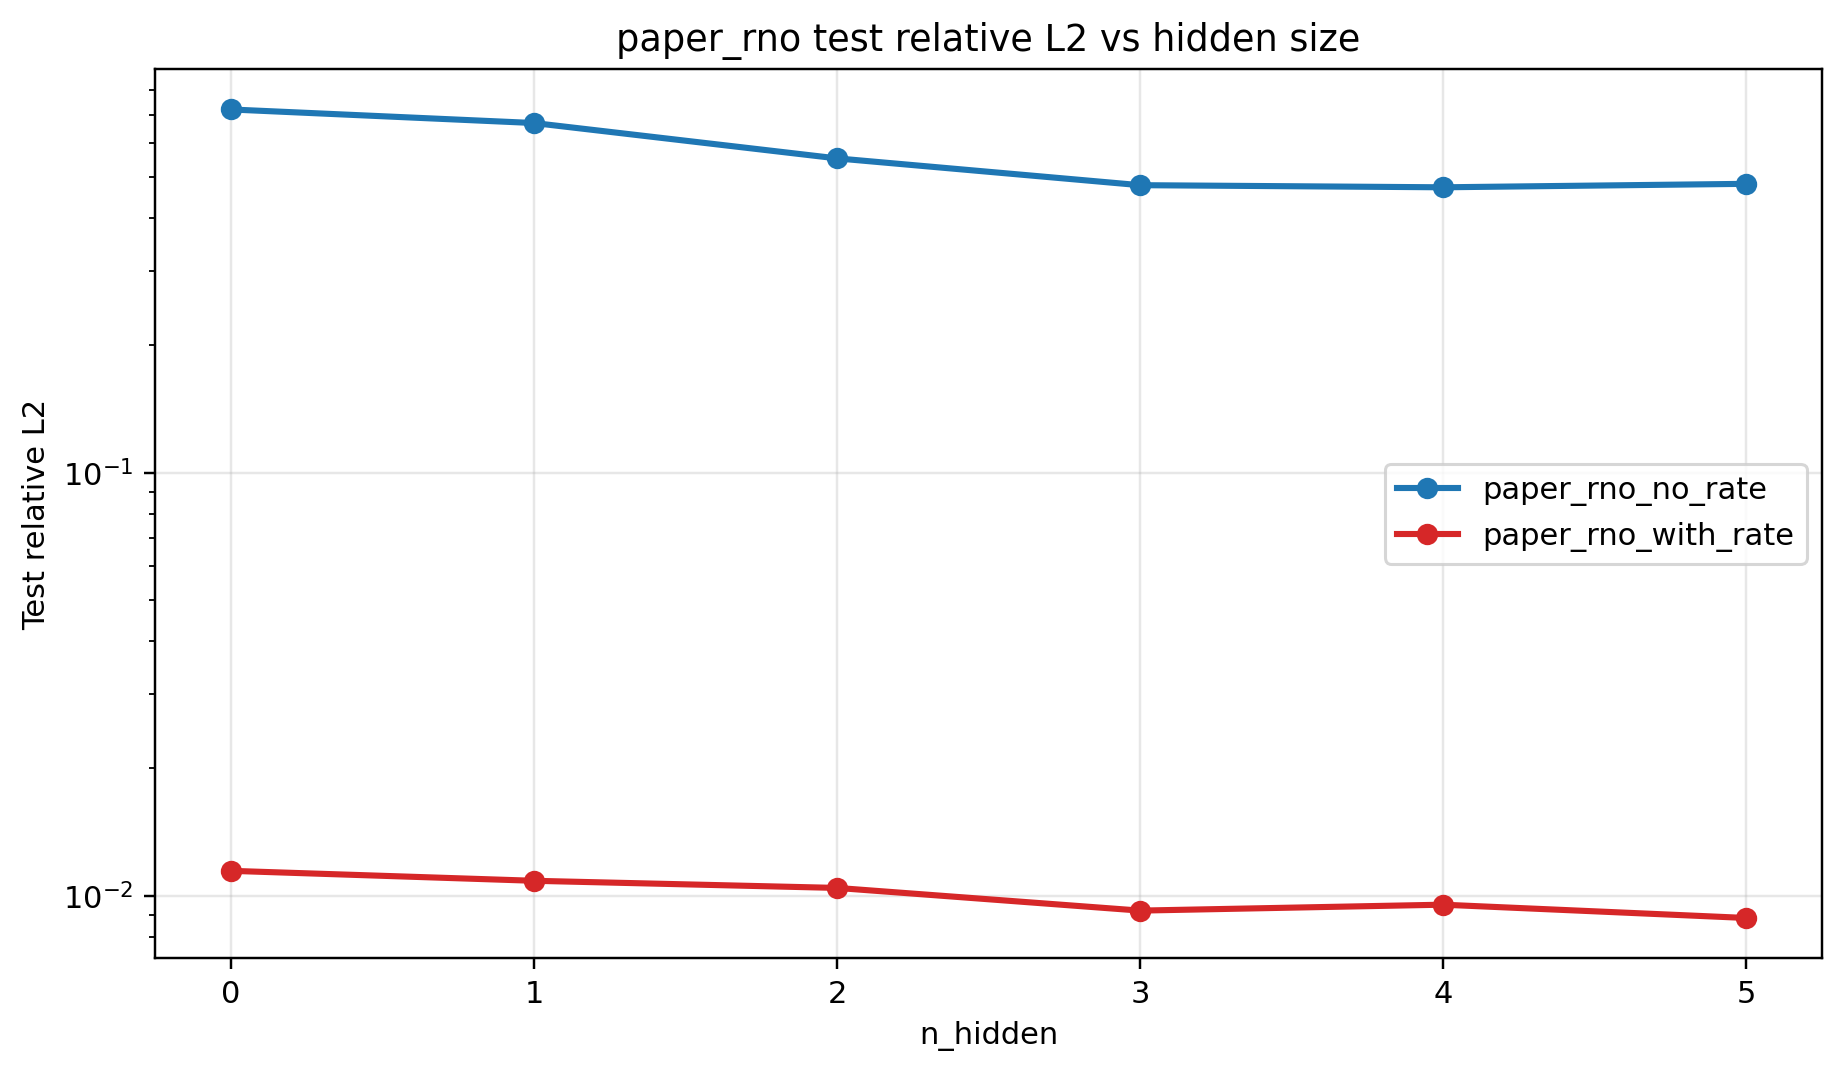
\includegraphics[width=\textwidth]{09_paper_rno_test_relative_l2_vs_hidden.png}
    \caption{Test relative $L^2$ against hidden dimension.}
\end{subfigure}
\caption{Paper-inspired hidden-size sweeps for the no-rate and with-rate variants. The no-rate model reveals the clearest threshold-like behaviour, while the with-rate model remains accurate across the full sweep and shows a much smoother dependence on hidden size.}
\label{fig:paper_hidden_sweeps}
\end{figure}

The threshold-style summaries for the two paper-inspired sweeps are shown separately in Figure~\ref{fig:paper_threshold_views}. For the no-rate model, the smallest hidden size within $5\%$ of the best validation loss is $h=3$. For the with-rate model, the same operational rule selects $h=5$, but this should not be overinterpreted: the curve is smooth and the $h=0$ model is already strong, so the threshold is acting more like a best-tested model selector than like a sharp physical dimension count.

\begin{figure}[t]
\centering
\begin{subfigure}[t]{0.48\textwidth}
    \centering
    
\includegraphics[width=\textwidth]{09_paper_rno_no_rate_h0to5_threshold.png}
    \caption{No-rate paper RNO threshold view.}
\end{subfigure}
\hfill
\begin{subfigure}[t]{0.48\textwidth}
    \centering
    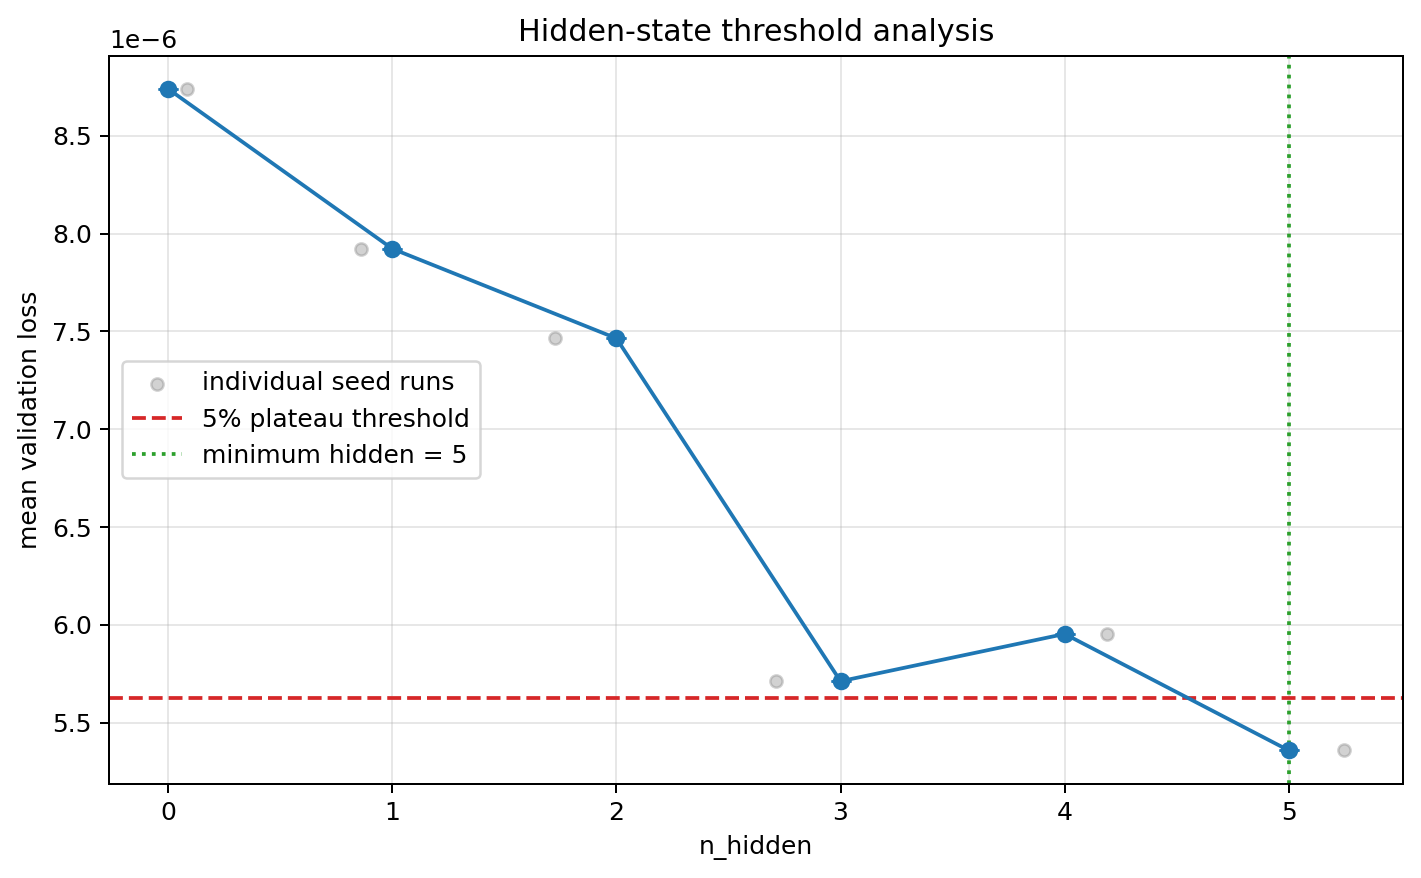
\includegraphics[width=\textwidth]{09_paper_rno_with_rate_h0to5_threshold.png}
    \caption{With-rate paper RNO threshold view.}
\end{subfigure}
\caption{Threshold-style summaries for the two paper-inspired sweeps. The no-rate model gives the clearest minimum hidden-size estimate, while the with-rate model remains accurate enough that the threshold criterion becomes much less decisive.}
\label{fig:paper_threshold_views}
\end{figure}

These results lead to a more nuanced answer to part (c) than a single universal integer. There is no architecture-independent threshold that emerges across every model. Instead:
\begin{enumerate}[leftmargin=1.5em]
    \item the best predictive GRU does not show a sharp low-dimensional cliff,
    \item the baseline and paper-inspired RNOs are more interpretable for internal-variable analysis,
    \item the clearest threshold-like result occurs for the no-rate paper RNO, where $h\approx 3$ is the smallest hidden size within $5\%$ of the best validation loss.
\end{enumerate}

This $h\approx 3$ result is physically plausible but should still be interpreted carefully. Since the dataset comes from a three-phase composite, it is tempting to map one hidden variable to each phase. That interpretation is qualitatively attractive. However, for a one-dimensional three-phase Kelvin--Voigt series composite the strict first-principles state count is closer to two independent internal variables after subtracting the observable macroscopic strain. The empirical value $h\approx 3$ is therefore best viewed as being of the right order, but slightly inflated because the no-rate paper RNO is compensating for omitted explicit rate information through its hidden state.

\FloatBarrier
\subsection{Hidden-State Geometry And Redundancy}

To understand why large hidden sizes can still behave as if only a few latent directions matter, the hidden-state trajectories were extracted and analysed by PCA. Figure~\ref{fig:hidden_state_geometry} shows the explained-variance and correlation summaries. The main result is that the strongest models occupy a highly redundant latent space. The best GRU uses $40$ hidden channels, but the first two principal components already explain $99.21\%$ of the hidden-state variance. The baseline RNO is similar, with $99.14\%$ explained by the first two components. Even the paper RNO with rate and $h=5$ places $99.77\%$ of its variance in the first two components.

\begin{figure}[t]
\centering
\begin{subfigure}[t]{0.48\textwidth}
    \centering
    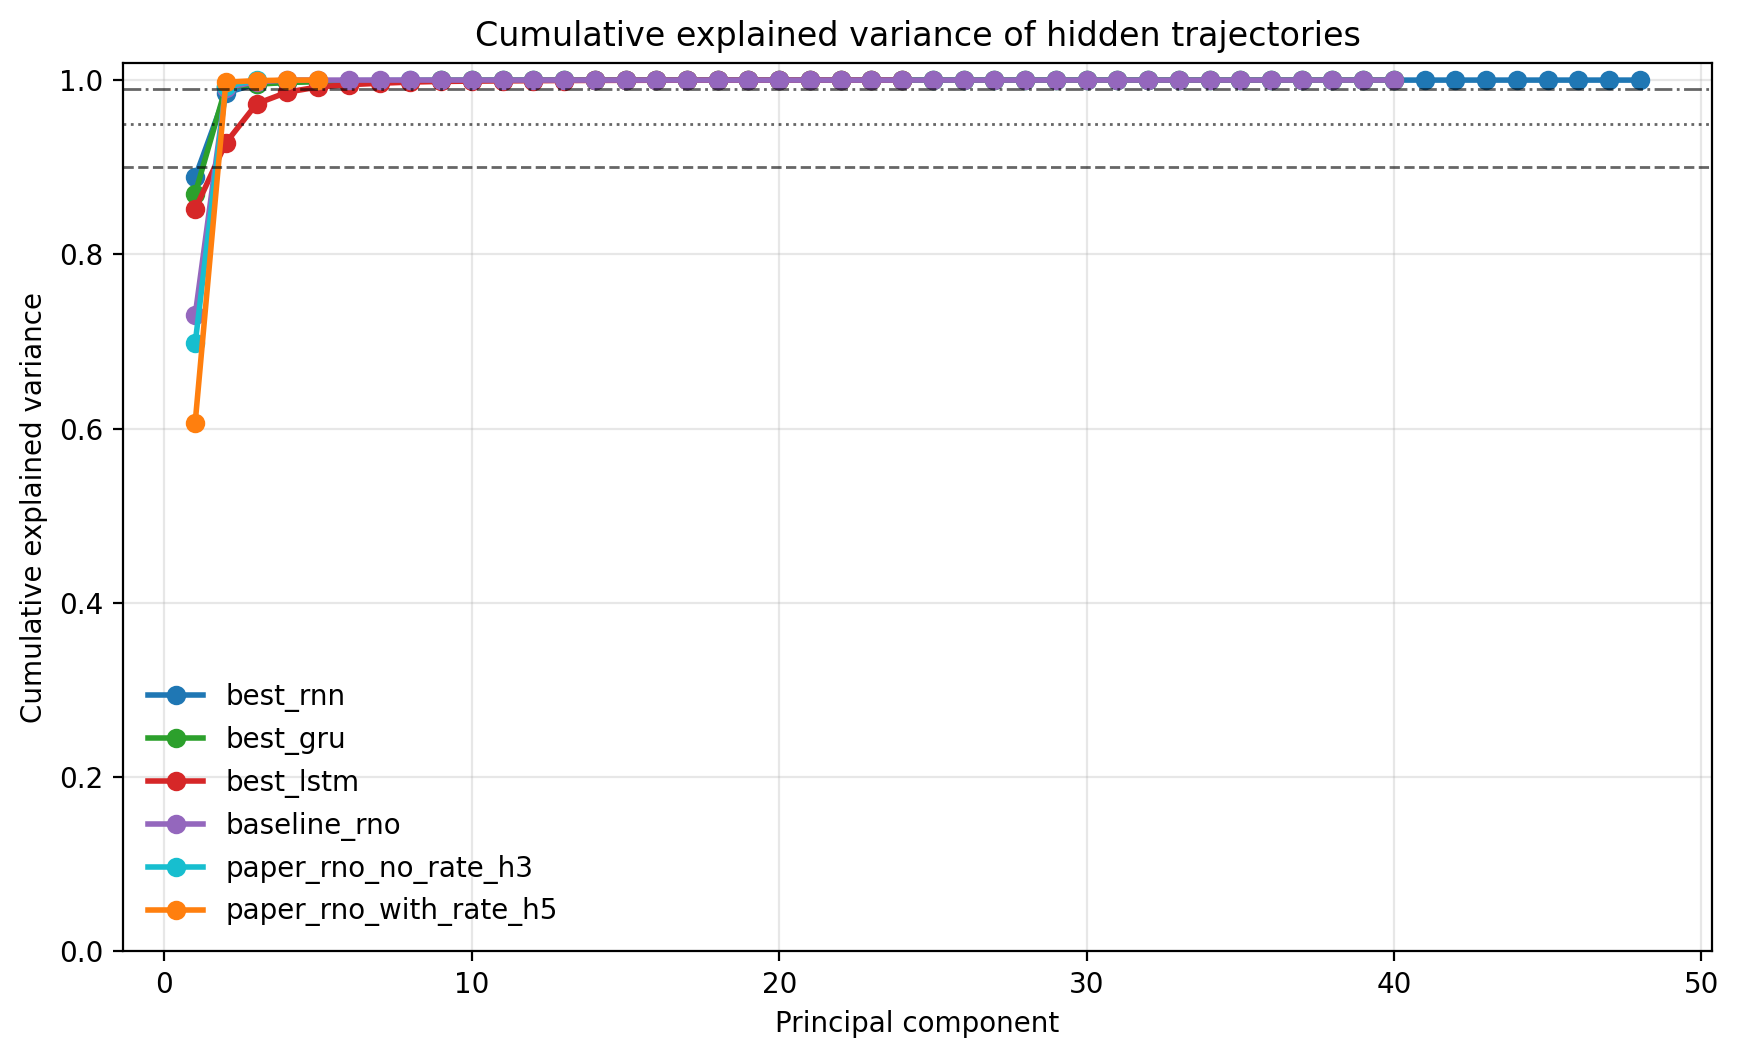
\includegraphics[width=\textwidth]{11_hidden_state_pca_explained_variance.png}
    \caption{PCA explained-variance curves for hidden trajectories.}
\end{subfigure}
\hfill
\begin{subfigure}[t]{0.48\textwidth}
    \centering
    
\includegraphics[width=\textwidth]{11_hidden_state_correlation_heatmaps.png}
    \caption{Hidden-state correlation heatmaps.}
\end{subfigure}
\caption{Hidden-state geometry for the trained models. High-performing models use latent spaces that are much more redundant than their raw hidden dimension suggests, with very strong pairwise correlations and very rapid PCA saturation.}
\label{fig:hidden_state_geometry}
\end{figure}

This observation helps explain the earlier threshold experiments. A large hidden size does not imply that the model is using all channels independently. In the cell-based models especially, many hidden channels collapse onto a low-dimensional manifold. That makes the mapping from ``hidden size'' to ``number of physical internal variables'' non-trivial. The dimensionality-reduction argument of Liu et al.~\cite{Liu_2023} is therefore useful as supporting evidence, but not as a standalone proof. Low latent dimensionality can coexist with both good and bad predictive performance. The paper-inspired no-rate model at $h=3$ is low dimensional, but is still much less accurate than the with-rate and GRU models because its constitutive inputs are more restricted.

\section{Discussion}

The most robust predictive conclusion of the project is that the GRU is the best macroscopic surrogate among the tested cell-based models. It achieves the lowest validation loss, the lowest test errors, and excellent qualitative behaviour on held-out and unseen loading paths. The baseline RNO is competitive, but not better than the GRU. This is a useful outcome in itself: the more structured state-space viewpoint improves interpretability, but the best black-box predictive model remains the gated recurrent architecture.

The more interesting scientific conclusion concerns part (c). A single universal threshold in hidden variables was \emph{not} observed across all architectures. This was not a failure of the investigation, but a finding about the models themselves. In the GRU and other rate-informed formulations, the model receives current strain, previous strain, and explicit strain rate, so the hidden state is not the sole carrier of constitutive memory. Under those conditions, $h=0$ can still perform surprisingly well, and the hidden-size curve becomes smooth rather than cliff-like.

The operator-inspired study clarifies this point. When the architecture is forced into the no-rate paper-style form, $h=0$ fails badly because the model reduces to an instantaneous constitutive map of current strain only. In that setting, a threshold-like improvement reappears and the smallest acceptable hidden dimension is about $3$. Once explicit strain rate is reintroduced, the threshold softens again and the performance becomes much less sensitive to hidden size. The hidden-state study therefore supports the following interpretation: explicit rate information is doing a large fraction of the constitutive work, while the latent hidden state supplies the remaining unresolved memory.

There is also a methodological lesson here. The model does not explicitly enforce thermodynamic restrictions such as convex stored energy or a dissipation inequality. Instead, it inherits physical plausibility from the high-fidelity data, which is the same pragmatic position taken by Liu et al.~\cite{Liu_2023}. This is adequate for the present coursework problem, but it also explains why hidden-state dimensions should be discussed cautiously: a good latent representation is not automatically the same thing as a physically unique internal-variable set.

Finally, the operator-style models retain one appealing theoretical property from the Liu framework: their hidden-state evolution is written as an explicit Euler step, so the architecture is naturally aware of the time increment $\dt$. This gives them a better claim to resolution independence than the purely cell-based models, although varying $\dt$ was not benchmarked directly here and should therefore be regarded as an architectural observation rather than an experimentally verified result in this report.

\section{Conclusion}

The coursework brief was addressed in three stages. First, the macroscopic constitutive input and output were defined as the strain-history-to-stress-history map in Equations~\eqref{eq:macro_operator} and~\eqref{eq:discrete_operator}. Second, recurrent surrogates were designed, trained, and compared. Optuna tuning showed that the GRU is the strongest predictive model on this dataset, achieving a best validation loss of $8.36\times 10^{-7}$ and a test relative $L^2$ error of $3.72\times 10^{-3}$. Third, the minimum hidden-variable question was investigated through progressively more constrained architectures.

The main answer to part (c) is therefore necessarily qualified. A single universal minimum hidden dimension was not found across all model classes. Instead, the threshold depends strongly on how much constitutive structure is provided explicitly in the inputs. The clearest threshold-like result arose in the paper-inspired no-rate RNO, where $h\approx 3$ was the smallest hidden size within $5\%$ of the best validation loss. However, once explicit strain rate was included, the dependence on hidden size became much smoother and the zero-hidden model was already strong. The most defensible conclusion is that the constitutive memory of this three-phase viscoelastic composite is low dimensional, but the observed minimum hidden size is architecture dependent and strongly affected by whether rate information is supplied explicitly.

\bibliographystyle{unsrt}
\bibliography{references}

\end{document}
